%
% introduction.tex
%
% Copyright The Radio Occultation Contributors.
%
% Radio Occultation Documentation
%
% This work is licensed under the Creative Commons Attribution-ShareAlike 4.0
% International License. To view a copy of this license,
% visit http://creativecommons.org/licenses/by-sa/4.0/.
%

%
% \brief Introduction chapter.
%
% \author Gabriel Mariano Marcelino <gabriel.mm8@gmail.com>
%
% \institution Universidade Federal de Santa Catarina (UFSC)
%
% \version 0.2.0
%
% \date 2020/06/05
%

\chapter{ \textcolor{red}{TODO} Introduction} \label{ch:introduction}

Radio Occultation is a 2U CubeSat (10$\times$10$\times$22.70 cm), and it is a follow up of Radio Occultation mission \cite{floripasat}. Both Radio Occultation and Radio Occultation are developed by SpaceLab/UFSC \cite{spacelab}. Radio Occultation main payload is the EDC board (\textit{Environmental Data Collection}) \cite{edc}, developed by INPE\nomenclature{\textbf{INPE}}{\textit{Instituto Nacional de Pesquisas Espaciais.}}. The mission is part of the ``GOLDS\nomenclature{\textbf{GOLDS}}{\textit{Global Open Collecting Data System.}}'' constellation (``Global Open Collecting Data System''), a collaborative CubeSat constellation for environmental data collection planned as part of the Brazilian Space Program \cite{golds}.

The project started just after the launch of Radio Occultation (first half of 2020) and is planned to be launched in 2023. Most of the embedded electronics is partially or totally based on the Radio Occultation satellite, with the same and/or improved versions of the modules. In other words, this project has, at some level, a flight heritage.

A conceptual image of the Radio Occultation satellite is shown in \autoref{fig:Radio Occultation-render}.

\begin{figure}[!ht]
    \begin{center}
        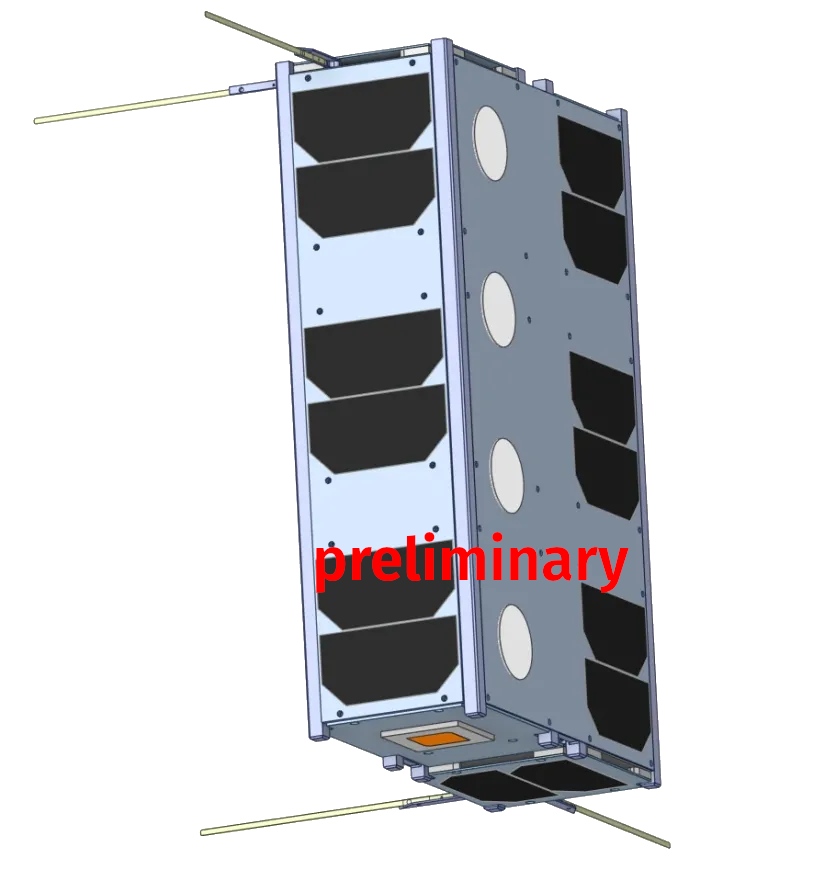
\includegraphics[width=0.8\textwidth]{figures/rocus-sat.png}
        \caption{Radio Occultation 3D renderization.}
        \label{fig:Radio Occultation-render}
    \end{center}
\end{figure}

\section{ \textcolor{red}{TODO} Mission Description}
The mission's main objective is the In-Orbit Validation (IoV) of INPE's EDC payload, using a service module based on Radio Occultation bus. The EDC payload is a module developed for CubeSats and capable of receiving data from data collection stations (Plataformas de Coleta de Dados, PCDs) of the Brazilian Data Collection System (\textit{Sistema Brasileiro de Coleta de Dados}, SBCD) installed along the Brazilian territory. The received data is forwarded to the ground segment through the main communication link offered by the satellite service module. A scientific contribution of the mission is the evaluation of radiation effects on electronic devices, as both EDC and the service platform are based on COTS. The radiation effects evaluation will be performed by the Radiation instrument, which has also been developed for the Radio Occultation mission. The mission provides also a relay service to the amateur radio community.
% The mission consists of testing the EDC payload developed by INPE in a real space mission, using for this, part of the flight heritage obtained during the Radio Occultation mission.

% The EDC payload is a module developed for CubeSats and capable of capturing data from data collection stations (PCDs) of the Brazilian Data Collection System (SBCD, or \textit{Sistema Brasileiro de Coleta de Dados}) installed along the Brazilian territory. The collected data can be retrieved through the main communication link offered by the satellite service modules. This mission will first use the EDC module in a space environment.

% As a secondary mission, we also intend to test other payloads, such as Payload-X, which is composed of a radiation-tolerant FPGA and a Radiation instrument using SRAM memories. These payloads, being secondary, will only be used for limited periods and upon request by telecommand.

\section{ \textcolor{red}{TODO} Mission Objectives}

The main objectives of the mission are as follows:

\begin{enumerate}
    \item In-Orbit Validation (IoV) of INPE's EDC payload.
    \item Provide a flight model for the satellite's service platform, based on Radio Occultation bus.
    \item Set up the ground segment for the mission operation.
    \item Receive environmental data from ground (from EDC stations), and forward the collected data to the ground station.
    \item Validate core-satellite functions in orbit.
    \item Perform experiments on radiation effects in electronic components in orbit, evaluating the radiation levels affecting EDC and the service platform modules.
    \item Serve as a relay for amateur radio communications, contributing to the amateur radio community.
\end{enumerate}

\section{ \textcolor{red}{TODO} Project Members}

All people involved in the project are students, professors and researchers from Federal University of Santa Catarina (UFSC), the National Institute for Space Research (INPE) and the Brazilian Space Agency (AEB\nomenclature{\textbf{AEB}}{\textit{Agência Espacial Brasileira.}}).

A list with the current members directly related to the project (2022/10/24) can be seen in \autoref{tab:team-members}.

\begin{table}[!htb]
    \centering
    \begin{tabular}{lllc}
        \toprule[1.5pt]
        \textbf{Name} & \textbf{Title} & \textbf{Position} & \textbf{Institution} \\
        \midrule
        Anderson Wedderhoff Spengler        & Dr.       & Professor             & UFSC \\
%        Edemar Morsch Filho                 & Dr.       & Professor             & UNESP \\
        Eduardo Augusto Bezerra             & Ph.D.     & Professor             & UFSC \\
        Richard Demo Souza                  & Dr.       & Professor             & UFSC \\
        Xisto Lucas Travassos               & Dr.       & Professor             & UFSC \\
        Laio Oriel Seman                    & Dr.       & Researcher            & UFSC \\
        Rodrigo Leonardi                    & Dr.       & Researcher            & AEB \\
        José Marcelo Duarte                 & Dr.       & Researcher            & INPE \\
        Manoel Jozeane Mafra de Carvalho    & M.Sc.     & Researcher            & INPE \\
        % Cezar Antônio Rigo                  & Dr.       & Researcher            & UFSC \\
        Gabriel Mariano Marcelino           & M.Sc.     & Doctoral Student      & UFSC \\
        Brenda Fernandes Ribeiro            & M.Sc.     & Doctoral Student      & UFSC \\
        André Martins Pio de Mattos         & B.Eng.    & Doctoral Student      & UFSC \\
        Edilberto Costa Neto                & B.Eng.    & Master Student      & UFSC \\
        Vinicius Pimenta Bernardo           & B.Eng.    & Master Student      & UFSC \\
        Augusto Cezar Boldori Vassoler      & B.Eng.    & Master Student      & UFSC \\
        % Amanda Medeiros                   & -         & Undergraduate Student & UFSC \\
        Bruno Benedetti                     & -         & Undergraduate Student & UFSC \\
        Caique Sales Miranda Gomes          & -         & Undergraduate Student & UFSC \\
        % Daniel Baron                      & -         & Undergraduate Student & UFSC \\
        João Cláudio Elsen Barcellos        & -         & Undergraduate Student & UFSC \\
        %Lorenzo Maturano                   & -         & Undergraduate Student & UFSC \\
        Lucas Zacchi                        & -         & Undergraduate Student & UFSC \\
        Matheus Wagner                      & -         & Undergraduate Student & UFSC \\
        %Maurício Sinigaglia                & -         & Undergraduate Student & UFSC \\
        Miguel Böing                        & -         & Undergraduate Student & UFSC \\
        Ramon de Araújo Borba               & -         & Undergraduate Student & UFSC \\
        % Tatiane dal Ross                  & -         & Undergraduate Student & UFSC \\
        Rebecca Quintino do O               & -         & Undergraduate Student & UFSC \\
        Vitória Beatriz Bianchin            & -         & Undergraduate Student & UFSC \\
        % Yan Castro de Azeredo             & -         & Undergraduate Student & UFSC \\
        \bottomrule[1.5pt]
    \end{tabular}
    \caption{Project members (2022/10/24).}
    \label{tab:team-members}
\end{table}

All the modules and methods used in this project are based in past works, mainly the Radio Occultation and the EDC projects. The list with the indirectly involved people is much bigger.

\section{ \textcolor{red}{TODO} Mission Patch}

The mission patch of the Radio Occultation can be seen in \autoref{fig:mission-patch}; it is inspired by the Radio Occultation patch \cite{floripasat} as it uses the flight heritage from its core modules (EPS, OBDH, TTC), which have been improved at hardware and/or software levels, to achieve the new requirements. The patch shows Brazil, the country of the mission's origin, gray orbits representing a constellation of CubeSats, and the yellow circles representing the "gold" color as a reference to the GOLDS constellation.

\begin{figure}[!htb]
    \begin{center}
        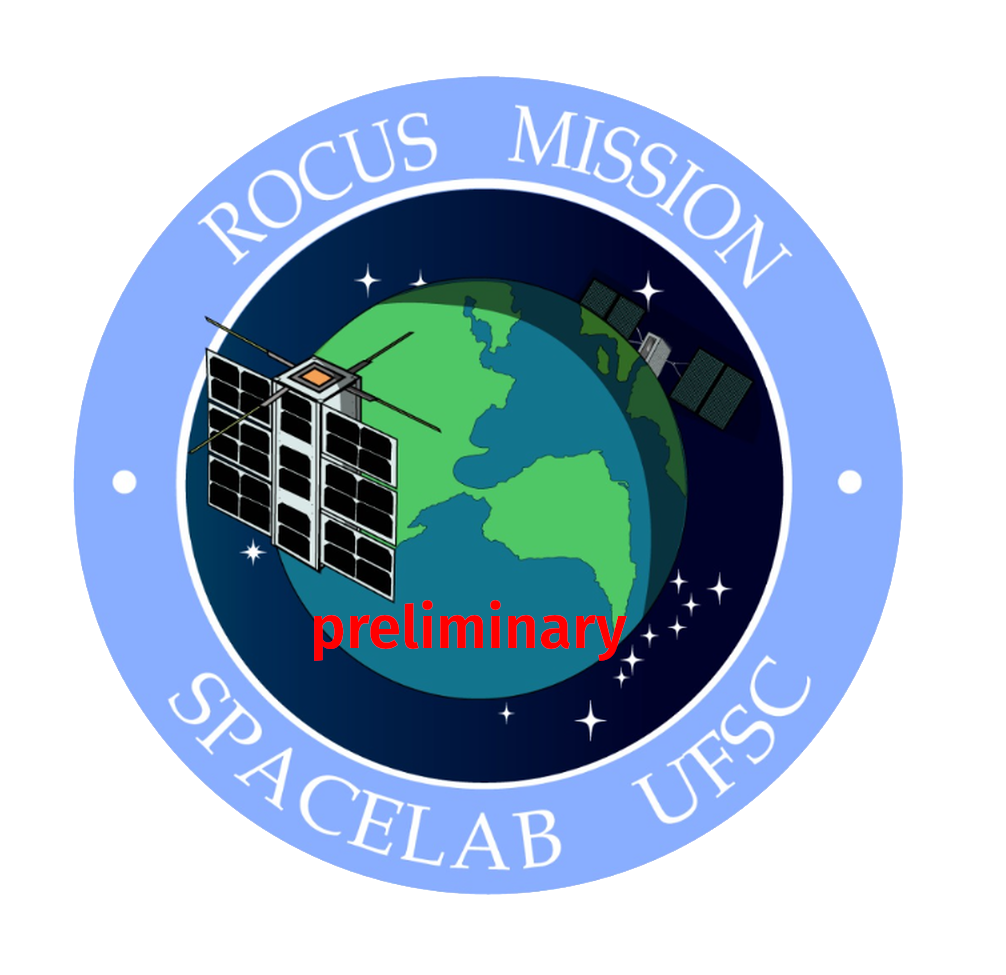
\includegraphics[width=0.5\textwidth]{figures/rocus-patch.png}
        \caption{Radio Occultation mission patch.}
        \label{fig:mission-patch}
    \end{center}
\end{figure}
